% ##############################################################################
% ##############################################################################
% #######   PLANTILLA FODAMI CAIM-CAIFE 2025                            ######## 
% #######   Creado con TeXstudio v 4.8.6   (c/archivo .cls)             ########
% #######   Autores: Equipo FIE - EAS|EAH|SEM                           ########
% ##############################################################################
\documentclass[a4paper]{fodami}        % customizado en archivo .cls    ########
%\usepackage{showframe}                % show layout de página (opt)    ########
% ##############################################################################
% ##############################################################################

% ---------- TÍTULO ------------------------------------------------------------
\title{\textbf{INTRODUCCIÓN TEMPRANA DE LA MECÁNICA COMPUTACIONAL EN CURSOS DE ELECTROSTÁTICA Y MECÁNICA ANALÍTICA}}

% ---------- AUTORES -----------------------------------------------------------
\author[1*]  {\textbf{Víctor A. Bettachini}}
\author[2,3]{\textbf{Mariano A. Real}}
\author[4]{\textbf{Edgardo Palazzo}}

% ---------- AFILIACIÓN --------------------------------------------------------
\setlength\parindent{0pt}
\affil[1]{Departamento de Ingeniería e Investigaciones Tecnológicas, Universidad Nacional de La Matanza (DIIT-UNLaM), Florencio Varela 1903, B1754JEC San Justo,Buenos Aires, Argentina.}
% \affil[1]{Departamento Académico de Mecánica, UTN - Facultad Regional Santa Fe, Lavaisse 610, 3000 Santa Fe, Argentina.}

\affil[2]{Instituto de Calidad Industrial, Universidad Nacional de San Martín - Instituto Nacional de Tecnología Industrial (INCALIN UNSaM-INTI), Av. General Paz 5445, B1684EFA Villa Martelli, Buenos Aires, Argentina.}

\affil[4]{Departamento de Materias Básicas, Universidad Tecnológica Nacional - Facultad Regional Avellaneda (UTN-FRA), Ramón Franco 5050, B1876ABY Villa Domínico, Buenos Aires, Argentina}

\affil[*]{Email: vbettachini@unlam.edu.ar}


% ##############################################################################
\begin{document}
\date{}

% ########## ENCABEZAMIENTOS y PIE #############################################
\renewcommand{\headrulewidth}{0pt} \renewcommand{\footrulewidth}{0pt}
\pagestyle{fancy}
\fancyhead{}
\fancyhead[C]{
	
\includegraphics[width=11.5cm]{imagenes/logoFODAMICAIMCAIFE.pdf}
	\noindent
	{\color{lightgray} \rule{\linewidth}{0.14cm}}
}
\fancyfoot{}
\fancyfootoffset[L]{-4cm}
\fancyfoot[L]{\footnotesize \flushleft \emph{IX CAIM 2025 - Noveno Congreso Argentino de Ingeniería Mecánica \\  
	IV CAIFE 2025 - Cuarto Congreso Argentino de Ingeniería Ferroviaria} \\
	\url{www.fie.undef.edu.ar/caimcaife2025} |  \href{mailto:caimcaife2025@fie.undef.edu.ar}{caimcaife2025@fie.undef.edu.ar}}
\setlength{\parskip}{8pt}
% ##############################################################################
	
\maketitle
\thispagestyle{fancy}

% ---------- RESUMEN -----------------------------------------------------------
\section*{
	\begin{center}
		RESUMEN
	\end{center}}
\vspace{-1.0cm}

Este trabajo presenta dos experiencias educativas que integran herramientas computacionales en la enseñanza de física para ingeniería, abordando desafíos comunes en entornos con recursos limitados.

La primera propuesta desarrolló un curso de mecánica analítica basado en Python, utilizando Jupyter notebooks y un enfoque de aula invertida. Los estudiantes resuelven ecuaciones de Euler-Lagrange mediante bibliotecas como SymPy y SciPy, centrándose en el modelado físico y evitando simplificaciones pedagógicas. El curso, disponible en GitHub, ha demostrado eficacia en grupos pequeños, aunque requiere adaptaciones para escalabilidad.

La segunda experiencia aplicó metodologías similares en electrostática, permitiendo a alumnos analizar distribuciones de carga continuas mediante cálculos simbólicos y numéricos en Google Colaboratory. Los resultados destacan una mayor comprensión conceptual sin depender de técnicas matemáticas avanzadas.

Ambos casos subrayan cómo la programación accesible (Python) y entornos interactivos (Jupyter) optimizan el tiempo en clase, priorizando el análisis sobre cálculos repetitivos, y ofrecen soluciones viables para instituciones con restricciones presupuestarias o logísticas. Estas estrategias, replicables y de código abierto, podrían extenderse a otras áreas de la física e ingeniería, potenciando el aprendizaje activo en contextos diversos.



% Este documento debe utilizarse como plantilla para el trabajo completo a presentar en el IX Congreso Argentino de Ingeniería Mecánica / IV Congreso Argentino de Ingeniería Ferroviaria. Contiene la estructura y formatos de texto.\\
% La primera página solo debe contener el Título, los Autores (hasta 6), la filiación, el Resumen y las Palabras clave. \textbf{El TÍTULO DEL TRABAJO}, en letra Arial 12 Mayúsculas Negrita, centrado, distanciado del encabezado por cuatro renglones de 12 pts. Con un renglón de separación se incluyen los autores del trabajo, identificados con el primer nombre, la inicial del segundo nombre y el apellido, en \textbf{ARIAL 10 negrita} centrados. Si la cantidad de autores ocupa mas de un renglón, entre ellos interlineado sencillo, y el último renglón con espaciado posterior 6pt. A continuación, en el renglón siguiente se indican las instituciones de los autores, sin repetirlas y con las correspondientes direcciones postales (en Arial 10) referidas con superíndices numéricos en los Apellidos. En el reglón siguiente, se debe indicar el e-mail del “autor de contacto” indicado con superíndice asterisco “*” en el listado de autores. \\
% Luego debe ir centrada la palabra \textbf{RESUMEN}, en Arial 10 negrita mayúscula, con un espaciado anterior de 24 pt y posterior de 6 pt. 
% El texto del resumen se escribe en Arial 10, con interlineado sencillo, sin espaciado entre párrafos, y alineación justificada. El mismo deberá contener el objetivo del trabajo, la metodología, resultados y conclusiones, sin superar las 300 palabras. En el trabajo completo, el resumen podrá tener diferencias respecto del aceptado originalmente, en la medida que no altere la naturaleza del objetivo del trabajo. \\
%A continuación, dejando un espacio de (10 pt.), se deben incluir las palabras clave, hasta un máximo de cuatro (4), en Arial 10 cursiva, con la primera letra de cada palabra en mayúscula.


\textit{\textbf{Palabras claves}: ?; ?; Ingeniería Mecánica; ?.}
% \textit{\textbf{Palabras claves}: Formato Trabajo; Congreso; Ingeniería Mecánica; Ingeniería Ferroviaria.}
	
% ---------- CUERPO del DOCUMENTO ----------------------------------------------
\newpage
\onehalfspacing
\setlength{\parskip}{0pt}
% ------------------------------------------------------------------------------

\section{INTRODUCCIÓN}




\paragraph{Mecánica computacional en asignaturas de física}
En las carreras de ingeniería las asignaturas de física tienen por correlativas previas asignaturas de matemática, e inmediatamente posteriores asignaturas donde se aplican algunos de estos conceptos en sistemas simples de la carrera de ingeniería en cuestión.
Como muestra el ejemplo de la figura \ref{fig:correlativasUNLaM}, en una asignatura de mecánica se aplican a asignaturas de mecánica de fluidos,  
De manera similar en una de electrónica, previo a los primeros cursos de circuitos se trata de explicar el funcionamiento de dispositivos electrónicos discretos fundamentados en la mecánica cuántica y electrostática con base en lo visto en asignaturas de física moderna y electromagnetismo.

\begin{figure}[ht]
	\centering
	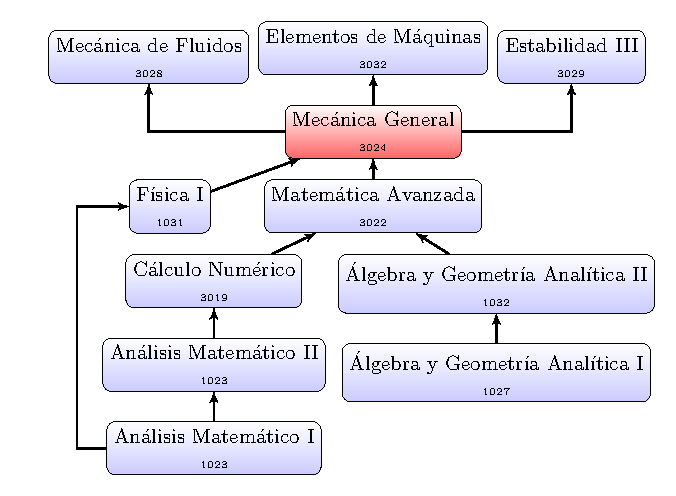
\includegraphics[width=0.6\textwidth]{../figuras/correlativas.pdf}
	\caption{
		Correlativas de la asignatura ``Mecánica general'' de la carrera de ingeniería mecánica de la UNLaM.
		Este curso de mecánica analítica es el umbral entre los otros de física y matemática hacia los más específicos de la carrera.  
		}
	\label{fig:correlativasUNLaM}
\end{figure}




Pero hay un salto grande en el nivel de complejidad entre la física que se enseña en los cursos de física y la física que se aplica en los cursos de ingeniería.


\paragraph{Aprovechar código no es programar}


\paragraph{El código es el mejor acople con LLMs}




En la tercera década del siglo veintiuno los cursos de ingeniería de las universidades latinoamericanas tienen aún como herramientas centrales el pizarrón y el papel.
Aun cuando docentes utilicen computadoras con proyectores y los alumnos escriban sus anotaciones en computadoras portátiles, se está reproduciendo el mismo esquema de enseñanza que se utiliza desde el siglo diecinueve; el docente presenta un tema, lo explica y los alumnos toman apuntes.

Esta sub explotación del medio digital queda aún más desactualizada en el contexto de una omnipresencia creciente de grandes modelos de lenguaje (LLM) como ChatGPT o DeepSeek, que permiten a los estudiantes obtener una rápida orientación sobre la temática que se está tratando.  
Entendemos que no es viable pretender que puede escindirse la ejercitación en los cursos de ingeniería del uso de LLM.
Por el contrario hoy es más acuciante 

Insistir con sustratos de papel y pizarrones incompatibles con los LLM es sumar otra tarea de transcripción a la que ya se condena a alumnos en el clásico esquema de tomar apuntes.

En este trabajo comentamos nuestra experiencia en la utilización de código como herramienta eje de la enseñanza de la ingeniería.
Nuestros cursos son de física para la ingeniería, y en particular de mecánica analítica y electrostática.



Todo sistema a analizar en el aula debe trabajarse en el marco de la mecánica computacional.
Esta disciplina conjuga la matemática, las distintas ramas de la física y herramientas de ciencias de la computación para explicar y modificar las relaciones entre la dinámica que presentan sistemas de objetos físicos de diversa composición ante diversos forzantes externos.  







\section{METODOLOGÍA PEDAGÓGICA CENTRADA EN LA MECÁNICA COMPUTACIONAL}





\subsection{Mecánica computacional para abordar más complejidad}

\subsection{Escribir código no es programar}

Si nos proponemos hacer mecánica computacional en un curso de grado de ingeniería, puede resultar tentador usar algún paquete de software específico para resolver problemas de física, que permita modelizar y simular sistemas utilizando alguna interfaz gráfica.
O por el contrario, utilizar un paquete de software más específico de matemática computacional, como Mathematica o Matlab.

Entendemos que para que la propuesta pueda ser transversal a varias temáticas debe utilizar una herramienta aun más general. 





\subsection{Los recursos están: plataformas en línea}

Se ha argumentado que las universidades públicas latinoamericanas al enfrentar las restricciones simultáneas de presupuestos ajustados y la necesidad de acomodar los horarios de sus clases a estudiantes que trabajan de día a horarios vespertinos, no cuentan con recursos informáticos para destinar a cursos que no estén directamente relacionados con la informática o la programación 
\cite{vallejo_google_2022}.%[@vallejo_google_2022:2022].




\section{CURSO DE MECÁNICA ANALÍTICA}

\subsection{Los recursos informáticos están: plataformas en línea}


\subsection{El docente no está para dar conferencias: aula invertida}




El curso aborda estas cuestiones proporcionando un entorno de aprendizaje gratuito, en línea y asíncrono que permite a los alumnos estudiar a su propio ritmo mediante el enfoque de aula invertida (flipped classroom) \cite{moraros_flipping_2015}.
%[@moraros_flipping_2015:2015].
Antes de las reuniones semanales, los alumnos deben estudiar la teoría y los ejemplos proporcionados en los cuadernos, así como iniciar la resolución de los ejercicios que los acompañan.
Durante esas reuniones vespertinas, ya sean en línea o presenciales, se anima a los alumnos a que formulen preguntas y comenten con el profesorado los problemas que no hayan podido resolver.

\begin{figure}[ht]
	\centering
	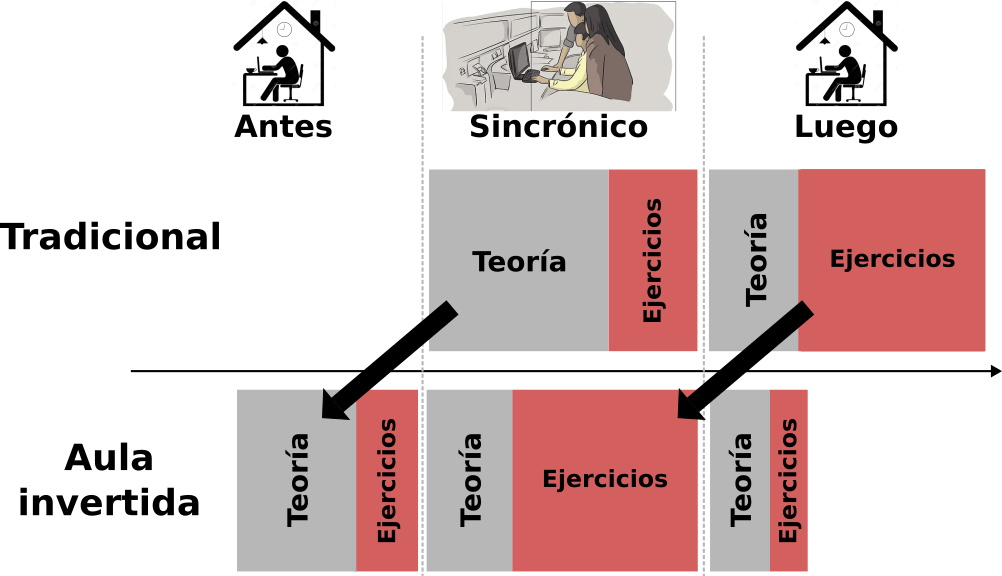
\includegraphics[width=0.6\textwidth]{../figuras/flippedClassroomSchedule_castellano.png}
	\caption{En esta implementación del aula invertida el alumno leer e intenta aplicar nueva teoría antes del encuentro sincrónico con el docente.
	Este se reserva a resolver dudas y discutir los problemas que no se han podido resolver.}
	\label{fig:flippedClassroomSchedule}
\end{figure}


\section{CURSO DE INTRODUCCIÓN A LA ELECTROSTÁTICA}

% \section{CURSO DE ELECTROSTÁTICA ELEMENTAL}



% ------------------------------------------------------------------------------
\section{CONCLUSIONES}
%Se apreciará que las mismas evidencien solidez y coherencia. Pueden incluirse en ellas otras cuestiones, como, por ejemplo, mención de interrogantes no dilucidados que podrían ser abordados en el futuro.

% ------------------------------------------------------------------------------
\section{AGRADECIMIENTOS}
% Adicionalmente, puede incluirse un apartado dedicado a los agradecimientos a personas o instituciones que han contribuido para la realización y/o financiación del trabajo.

Los autores de este trabajo desean agradecer a DIIT-UNLaM por su apoyo al trabajo aquí reportado que es parte de los proyectos C2-ING-109 (2023-2024) y C2-ING-143 (2025-2026), este último parte del Programa de Investigación Mejora de las Estrategias Pedagógicas dirigido por la Dra. Bettina Donadelllo.
Ambos proyectos están acreditados en el Programa de Investigación Científica, Desarrollo y Transferencia de Tecnología e Innovaciones (CyTMA2) de la mencionada institución.

% -----------------------------------------------------------------------------	
\section{REFERENCIAS}

%Se considera valioso incluir menciones a textos y artículos de publicaciones reconocidas, valorándose la incorporación de aquellas de reciente edición. La forma de indicar las citas bibliográficas en el texto está especificada al final de la sección \textbf{1. INTRODUCCIÓN}. Solamente deben incluirse las referencias citadas en el cuerpo del documento, según su orden de aparición. El formato de las referencias según \textbf{Normas APA (7ª edición, 2024)}. A continuación, se brindan algunos ejemplos:
%
%\textbf{1. Libro} \cite{budynas_diseno_2012}
%
%[1] Apellido, A. A. y Apellido, B.B. (Año). Título del libro en cursiva. Edición. Editorial.
%
%\textit{\textbf{Ejemplo:}}
%\begin{enumerate}[label={[}\arabic*{]}]
%	\item Budynas, R.G. and Nisbett, J. K.  (2012). \textit{Shigley's Mechanical Engineering Design}. 9th Ed. McGraw-Hill.
%\end{enumerate}
%
%\textbf{2. Artículo de revista} \cite{moreno_abandono_2019}
%
%[2] Apellido, A.A. y Apellido, B.B. (Año). Título del artículo. Título de la revista en cursiva, volumen(número), páginas. https://doi.org/xxxx (si está disponible).
%
%\textit{\textbf{Ejemplo:}}
%\begin{enumerate}[label={[}\arabic*{]}]
%	\setcounter{enumi}{1}
%	\item Moreno J. and Chiecher A., (2019). \textit{Dropout in Engineering careers. A study of academic, socio-demographic, labor and life aspects}. Educational Research Notebooks, 10, (2),73-90, DOI:\\ https://doi.org/10.18861/cied.2019.10.2.2908
%\end{enumerate}
%
%
%\textbf{3. Artículo en línea} \cite{lu_aprobarias_2015}
%
%[3] Apellido, A. A. (Año). Título del artículo. Nombre del sitio web. URL
%
%\textit{\textbf{Ejemplo:}}
%\begin{enumerate}[label={[}\arabic*{]}]
%	\setcounter{enumi}{2}
%	\item Lu S. and Whiteman H. (2015) \textit{¿Would you pass the college entrance exam in China?}, CNN in espanish.\\
%	https://cnnespanol.cnn.com/2015/06/09/aprobarias-el-examen-de-ingreso-a-la-universidad-en-china
%\end{enumerate}
%
%\textbf{4. Informe o documento institucional} \cite{organizacion_mundial_de_la_salud_informe_2020}
%
%[4] Nombre de la institución. (Año). Título del informe en cursiva. URL (si aplica)
%
%\textit{\textbf{Ejemplo:}}
%\begin{enumerate}[label={[}\arabic*{]}]
%	\setcounter{enumi}{3}
%	\item World Health Organization. (2020). \textit{The World Mental Health Report}.\\
%	https://www.who.int/informes/saludmental2020
%\end{enumerate}
%
%\textbf{5. Tesis o disertación} \cite{jerez_resultados_2012}
%
%[5] Apellido, A. A. (Año). Título de la tesis o disertación en cursiva (Tesis doctoral, Nombre de la Institución que otorga el título). Nombre de la base de datos. URL (si está disponible)
%
%\textit{\textbf{Ejemplo:}}
%\begin{enumerate}[label={[}\arabic*{]}]
%	\setcounter{enumi}{4}
%	\item Jerez, O., (2012), \textit{Los resultados de aprendizaje en la Educación Superior por Competencias}. Doctoral Thesis, University of Granada, Spain. ISSN: 978-84-695.1027-8. https://dialnet.unirioja.es/servlet/tesis?codigo=62470
%\end{enumerate}
%
%\textbf{6. Norma o estándar} \cite{noauthor_iso_2020}
%
%[6] Nombre del organismo. (Año). Título de la norma en cursiva (Código y número de la norma). Editorial (si aplica). URL (si se obtuvo en línea).
%
%\textit{\textbf{Ejemplo:}}
%\begin{enumerate}[label={[}\arabic*{]}]
%	\setcounter{enumi}{5}
%	\item International Organization for Standardization. (2020). ISO 9001:2015: \textit{Sistemas de gestión de la calidad (Norma Internacional 9001)}.
%\end{enumerate}	
%
%\textbf{7. Trabajo presentado en un congreso o conferencia} \cite{xiaobin_stress_2013}
%
%[7] Apellido, A. A., y Apellido, N. T. (Año). Título del trabajo. Denominación del Congreso, Registro (ISBN o ISSN), Lugar y fechas.
%
%\textit{\textbf{Ejemplo:}}
%\begin{enumerate}[label={[}\arabic*{]}]
%	\setcounter{enumi}{6}
%	\item Xiaobin L. y Zelong L. (2013). \textit{Stress concentration factors due to typical geometric discontinuities for shaft design by numerical simulation}. ASEE Annual Conference and Exposition, Atlanta, Georgia, June 23-26, 2013, DOI 10.18260/1-2—22476 
%\end{enumerate}
%
%{\color{gray} \rule{\linewidth}{0.5pt}}
%\textbf{Pautas importantes:}
%\begin{itemize}
%	\item \textbf{Cursiva}: Los títulos de libros y de revistas, denominación de congreso y normas deben ir en cursiva.
%	\item \textbf{DOI}: Si un artículo tiene un DOI, debe incluirse al final de la referencia.
%	\item \textbf{URL}: En el caso de las fuentes en línea, incluye la URL completa, con texto en color negro sin formato de hipervínculo. No aplica ``Recuperado de'' a menos que sea necesario (por ejemplo, si la fecha de acceso es relevante).
%\end{itemize}
%
% ------------------------------------------------------------------------------
\renewcommand{\bibname}{Referencias}% cambio de nombre
%\nocite{*}
\printbibliography


\end{document}

% ##############################################################################
% ##############################################################################
